% Author: Victor Terron (c) 2013
% Email: `echo vt2rron1iaa32s | tr 132 @.e`
% License: GNU GPLv3

\documentclass[14pt]{beamer}

\usepackage[utf8]{inputenc}
\usepackage{listings}
\usepackage[T1]{fontenc}

% Reduce space between image and caption; also remove prefix 'Figure:'
% http://tex.stackexchange.com/a/94018
% http://tex.stackexchange.com/a/82462
\usepackage[font=small,skip=1pt,labelformat=empty]{caption}

\usetheme{Copenhagen}
\useoutertheme{infolines}
\setbeamercovered{dynamic}
\setbeamertemplate{navigation symbols}{} % remove navigation symbols

\lstset{basicstyle=\ttfamily,language=python}

% Remove the space symbol for code inside the double quotation marks
% http://www.latex-community.org/viewtopic.php?f=4&t=248
\lstset{showstringspaces=false}

\title{Cuarenta características de Python\\ que quizás no conoces}
\author{Víctor Terrón}
\date{23 de noviembre de 2013}
\institute{IAA-CSIC}

\begin{document}

\begin{frame}
  \titlepage
  \begin{figure}
    \vspace{-0.5cm}
    
\includegraphics[width=3cm]{pics/mistery-box.jpg}
  \end{figure}
\end{frame}

\section{Introducción}

\begin{frame}{Unknown Unknowns}
  \small
  \begin{block}{}
    \centering
    ``There are things we know that we know. There are known
    unknowns. That is to say there are things that we now know we
    don't know. But there are also \structure{unknown unknowns}. There
    are things we do not know we don't know'' [Donald Rumsfeld, 2002]
  \end{block}

  \small
  \begin{itemize}
    \item En Python hay funcionalidades increíbles,
     \structure{imprescindibles una vez que las conoces}, que
     podríamos no echar en falta jamás porque ni siquiera sabíamos
     que existían.
    \item El propósito de esta charla es presentar una serie de
      aspectos interesantes de Python que en estos años he descubierto
      que mucha gente, incluso programadores veteranos, desconoce.
  \end{itemize}
\end{frame}

\begin{frame}{Unknown Unknowns}
  \begin{itemize}
    \item Algunas de las funcionalidades que vamos a discutir aquí son
      muy prácticas y otras curiosidades de indiscutiblemente escasa o
      nula utilidad en nuestro día a día. Pero todos ellos son
      conceptos \structure{sencillos de entender} y que merece la pena
      saber que están ahí, incluso si no los usamos... por ahora.
    \item Tenemos 1:15 minutos para cada uno de los puntos, así que
      muchos de ellos sólo vamos a poder \structure{verlos muy por
      encima}. Pero al menos habrán dejado de ser \emph{unknown
      unknowns}.
  \end{itemize}
\end{frame}

\begin{frame}{¡No os limitéis a escuchar!}
  \begin{center}
    No suele ser divertido escuchar a nadie hablar durante casi una
    hora. Participad, intervenid, criticad, opinad. ¡Si digo algo que
    no tiene ningún sentido, \structure{corregidme}!
  \end{center}

  \begin{block}{\centering El código fuente está disponible en:}
    \centering \url{http://github.com/vterron/PyConES-2013}
  \end{block}

  \begin{center}
    \small Erratas, correcciones, enlaces interesantes...\\ ¿enviará
    alguien algún pull request antes de que termine esta charla?
  \end{center}
\end{frame}

\begin{frame}{}
  \begin{alertblock}{}
    \centering \Large ¿Listos?
  \end{alertblock}

  \begin{figure}
    \centering
    
\includegraphics[height=6cm]{pics/a-clockwork-orange.jpg}
  \end{figure}
\end{frame}

\begin{frame}[fragile]{1. Intercambiar dos variables}

  \begin{center}
    Normalmente, en otros lenguajes de programación, tenemos que usar
    una \structure{variable temporal} para almacenar uno de los dos
    valores.
  \end{center}

  \small
  \begin{exampleblock}{Por ejemplo, en C}
    \begin{lstlisting}[language=C]
int x, y;
int tmp;
tmp = x;
x = y;
y = x;
    \end{lstlisting}
  \end{exampleblock}
\end{frame}

\begin{frame}[fragile]{1. Intercambiar dos variables}
  \begin{block}{Python nos permite hacer}
    \centering \LARGE a, b = b, a
  \end{block}

  \begin{exampleblock}{}
    \begin{lstlisting}
>>> a = 5
>>> b = 7
>>> a, b = b, a
>>> a
7
>>> b
5
    \end{lstlisting}
  \end{exampleblock}
\end{frame}

\begin{frame}{1. Intercambiar dos variables}
  \begin{alertblock}{}
    \centering Desde nuestro punto de vista, ambas asignaciones
    ocurren simultáneamente. La clave está en que tanto \\
    \structure{a, b} como \structure{b, a} son \structure{tuplas}.
  \end{alertblock}

  Las expresiones en Python se evalúan de izquierda a derecha. En una
  asignación, el lado derecho se evalúa antes que el derecho. Por tanto:

  \begin{itemize}
    \item El lado derecho de la asignación es evaluado, creando una
      \structure{tupla de dos elementos} en memoria, cuyos elementos
      son los objetos designados por los identificadores \structure{b}
      y \structure{a}.
  \end{itemize}
\end{frame}

\begin{frame}{1. Intercambiar dos variables}
  \begin{itemize}
    \item El lado izquierdo es evaluado: Python ve que estamos
      asignando una tupla de dos elementos a otra tupla de dos
      elementos, así que \emph{desempaqueta} (\structure{tuple
        unpack}) la tupla y los asigna uno a uno:
      \begin{itemize}
        \item Al primer elemento de la tupla de la izquierda,
          \structure{a}, le asigna el primer elemento de la tupla que
          se ha creado en memoria a la derecha, el objeto que antes
          tenía el identificador \structure{b}. Así, el nuevo
          \structure{a} es el antiguo \structure{b}.
        \item Del mismo modo, el nuevo \structure{b} pasa a ser el
          antiguo \structure{a}.
      \end{itemize}
  \end{itemize}

  \small
  \begin{block}{Explicación detallada en Stack Overflow:}
    \centering \url{http://stackoverflow.com/a/14836456/184363}
  \end{block}
\end{frame}

\begin{frame}{1. Intercambiar dos variables}
  \begin{center}
    ¿Cómo se declara una tupla de \structure{un único elemento}?
  \end{center}

  \begin{block}{}
    \centering \huge 1,
  \end{block}

  o, para más claridad,

  \begin{block}{}
    \centering \huge (1,)
  \end{block}

  \begin{alertblock}{}
    \centering Es la \structure{coma}, no el paréntesis, el
    constructor de la tupla
  \end{alertblock}
\end{frame}

\begin{frame}[fragile]{1. Intercambiar dos variables}

  \small
  \begin{block}{}
    \centering Los paréntesis por sí mismos no crean una tupla: Python
    \structure{evalúa la expresión} dentro de los mismos y devuelve el
    valor resultante:
  \end{block}

  \small
  \begin{exampleblock}{Esto sólo suma dos números}
    \begin{lstlisting}
>>> 2 + (1)
3
    \end{lstlisting}
  \end{exampleblock}

  \begin{exampleblock}{Esto intenta sumar entero y tupla (y fracasa)} \scriptsize
    \begin{lstlisting}
>>> 2 + (1,)
Traceback (most recent call last):
  File "<stdin>", line 1, in <module>
TypeError: unsupported operand type(s) for +: 'int' and 'tuple'
    \end{lstlisting}
  \end{exampleblock}
\end{frame}

\begin{frame}{2. Encadenamiento de operadores lógicos}
  \begin{alertblock}{En vez de escribir}
    \centering \LARGE x => y and y < z
  \end{alertblock}

  \small
  \begin{center}
    A diferencia de C, todos los operadores lógicos tienen la misma
    prioridad, y pueden ser encadenados de forma arbitraria.
  \end{center}

  \begin{block}{Mucho mejor}
    \centering \LARGE x <= y < z
  \end{block}

  \small
  \begin{center}
    Las dos expresiones de arriba son equivalentes, aunque en la
    segunda \structure{x} sólo se evalúa una vez. En ambos casos,
    \structure{z} no llega a evaluarse si no se cumple que
    \structure{x <= y} (\emph{lazy evaluation}).
  \end{center}
\end{frame}

\begin{frame}[fragile]{3. 0.1 + 0.2 != 0.3}
  \begin{alertblock}{}
    \centering \Large ¿Por qué 0.1 + 0.2 == 0.3 es \structure{False}?
  \end{alertblock}

  \begin{exampleblock}{}
    \begin{lstlisting}
>>> 0.1 + 0.2 == 0.3
False
    \end{lstlisting}
  \end{exampleblock}

  \begin{center}
    Porque los números flotantes se representan internamente, en
    cualquier ordenador, como \structure{fracciones binarias}. Por
    ejemplo, 1.25 es equivalente a 1/2 + 3/4.
  \end{center}
\end{frame}

\begin{frame}[fragile]{3. 0.1 + 0.2 != 0.3}
  \footnotesize
  \begin{center}
    La mayor parte de las fracciones decimales no puede ser
    representada exactamente con una fracción binaria. Lo máximo que
    los números flotantes pueden hacer es \structure{aproximar su
    valor real} --- con bastantes decimales, pero nunca el exacto.
  \end{center}

  \begin{exampleblock}{}
    \small
    \begin{lstlisting}
>>> print "%.30f" % 0.1
0.100000000000000005551115123126
>>> print "%.30f" % 0.2
0.200000000000000011102230246252
>>> print "%.30f" % 0.3
0.299999999999999988897769753748
    \end{lstlisting}
  \end{exampleblock}

  \footnotesize
  \begin{center}
    Lo mismo ocurre en base decimal con, por ejemplo, el número
    1/3. Por más decimales con que se represente, 0.333333... no deja
    de ser una aproximación.
  \end{center}
\end{frame}

\begin{frame}[fragile]{3. 0.1 + 0.2 != 0.3}
  \small
  \begin{center}
    Normalmente no somos conscientes de esto porque Python por defecto
    nos muestra una aproximación del valor real de los números
    flotantes, redondeándolos a una \structure{representación
    práctica} para nosotros.
  \end{center}

  \begin{exampleblock}{}
    \small
    \begin{lstlisting}
>>> print 0.1
0.1
>>> print 0.2
0.2
>>> print 0.3
0.3
>>> 0.1 + 0.2
0.30000000000000004
    \end{lstlisting}
  \end{exampleblock}

  \small
  \begin{block}{Floating Point Arithmetic: Issues and Limitations}
    \centering \url{http://docs.python.org/2/tutorial/floatingpoint.html}
  \end{block}
\end{frame}

\begin{frame}[fragile]{3. 0.1 + 0.2 != 0.3}
  \begin{alertblock}{}
    \centering \small Nunca deberíamos comparar números flotantes
    directamente
  \end{alertblock}

  \small
  \begin{center}
    Una opción, simple, es comprobar si ambos valores son lo
    "\emph{suficientemente iguales}" usando un valor máximo de error
    absoluto admisible, normalmente llamado \structure{epsilon}.
   \end{center}

  \begin{exampleblock}{}
    \begin{lstlisting}
>>> epsilon = 1e-10
>>> abs((0.1 + 0.2) - 0.3) < epsilon
True
>>> abs((0.1 + 0.2) - 0.3)
5.5511151231257827e-17
    \end{lstlisting}
  \end{exampleblock}
\end{frame}

\begin{frame}{3. 0.1 + 0.2 != 0.3}
  \large
  \begin{center}
    En caso de no conocer el rango de los números con los que vamos a
    trabajar, tenemos que compararlos en términos de \structure{error
    relativo} \\ ("\emph{son iguales al 99.999\%}).
  \end{center}

  \small
  \begin{block}{Comparing Floating Point Numbers, 2012 Edition}
    \centering \url{http://randomascii.wordpress.com/2012/02/25/comparing-floating-point-numbers-2012-edition/}
  \end{block}
\end{frame}

\begin{frame}[fragile]{3. 0.1 + 0.2 != 0.3}
  \begin{block}{}
    \centering En Python tenemos el módulo \structure{decimal}
  \end{block}

  \begin{exampleblock}{}
    \begin{lstlisting}
>>> import decimal
>>> x = decimal.Decimal("0.1")
>>> y = decimal.Decimal("0.2")
>>> z = decimal.Decimal("0.3")
>>> x + y == z
True
    \end{lstlisting}
  \end{exampleblock}

  \small
  \begin{block}{decimal --- Decimal fixed point and floating point arithmetic}
    \centering \url{http://docs.python.org/2/library/decimal.html}
  \end{block}
\end{frame}

\begin{frame}[fragile]{4. int(True) == 1}
  \large
  \begin{alertblock}{}
    \centering
    El valor numérico de \structure{True} es 1; el de \structure{False}, 0
  \end{alertblock}

  \begin{exampleblock}{}
    \small
    \begin{lstlisting}
>>> int(True)
1
>>> int(False)
0
>>> 37 + True
38
>>> 7 / False
Traceback (most recent call last):
  File "<stdin>", line 1, in <module>
ZeroDivisionError: float division
    \end{lstlisting}
  \end{exampleblock}
\end{frame}

\begin{frame}[fragile]{4. int(True) == 1}
  \large
  \begin{block}{}
    \centering
    De hecho, la clase \structure{bool} hereda de \structure{int}
  \end{block}

  \begin{exampleblock}{}
    \small
    \begin{lstlisting}
>>> issubclass(bool, int)
True
>>> isinstance(True, int)
True
>>> bool.mro()
[<type 'bool'>, <type 'int'>, <type 'object'>]
    \end{lstlisting}
  \end{exampleblock}

  \small
  \begin{block}{\centering PEP 285: Adding a bool type [2002]}
    \centering \url{http://www.python.org/dev/peps/pep-0285/}
  \end{block}
\end{frame}

\begin{frame}[fragile]{5. import this}
  \Large
  \begin{block}{}
    \centering El Zen de Python
  \end{block}

  \begin{exampleblock}{\small Los principios filosóficos en los que se cimenta Python}
    \tiny
    \begin{lstlisting}
>>> import this
The Zen of Python, by Tim Peters

Beautiful is better than ugly.
Explicit is better than implicit.
Simple is better than complex.
Complex is better than complicated.
Flat is better than nested.
Sparse is better than dense.
Readability counts.
[...]
    \end{lstlisting}
  \end{exampleblock}

  \small
  \begin{block}{\centering PEP 20: The Zen of Python [2004]}
    \centering \url{http://www.python.org/dev/peps/pep-0020/}
  \end{block}
\end{frame}

\begin{frame}[fragile]{5. import this}
  \small
  \begin{center}
    Algo aún más desconocido: el contenido del módulo
    \structure{this.py} está cifrado con el algoritmo
    \structure{ROT13} --- cada letra sustituida por la que está trece
    posiciones por delante en el alfabeto:
  \end{center}

  \begin{exampleblock}{}
    \tiny
    \begin{lstlisting}
>>> import inspect
>>> print inspect.getsource(this)
s = """Gur Mra bs Clguba, ol Gvz Crgref

Ornhgvshy vf orggre guna htyl.
Rkcyvpvg vf orggre guna vzcyvpvg.
Fvzcyr vf orggre guna pbzcyrk.
Pbzcyrk vf orggre guna pbzcyvpngrq.
Syng vf orggre guna arfgrq.
Fcnefr vf orggre guna qrafr.
Ernqnovyvgl pbhagf.
[...]
    \end{lstlisting}
  \end{exampleblock}

  \scriptsize
  \begin{block}{\centering this and The Zen of Python}
    \centering
    \url{http://www.wefearchange.org/2010/06/import-this-and-zen-of-python.html}
  \end{block}
\end{frame}

\begin{frame}{6. El módulo antigravedad}
  \Large
  \begin{block}{}
    \centering import antigravity
  \end{block}{}

  \begin{figure}
    \centering
    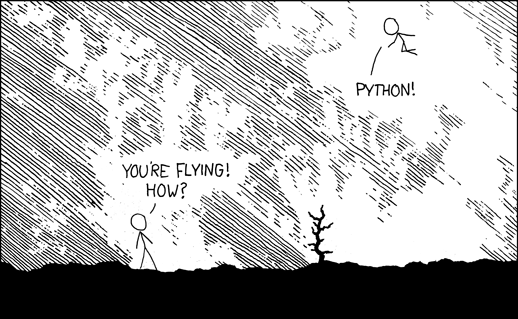
\includegraphics[height=4cm]{pics/xkcd-353.png}
    \caption{\url{http://xkcd.com/353/}}
  \end{figure}

  \vspace{-0.75cm}

  \small
  \begin{alertblock}{}
    \centering
    Añadido en Python 3, pero también está disponible en Python 2.7
  \end{alertblock}
\end{frame}

\begin{frame}[fragile]{6. El módulo antigravedad}
  \begin{exampleblock}{\small antigravity.py}
    \small
    \begin{lstlisting}
>>> print inspect.getsource(antigravity)
import webbrowser
webbrowser.open("http://xkcd.com/353/")
    \end{lstlisting}
  \end{exampleblock}

  \begin{center}
     \small
     En Py3K el módulo \structure{antigravity} incluye la función
     \structure{geohash()}, referencia a otra viñeta de XKCD en la que
     se describe un algoritmo que genera coodenadas en base a la fecha
     y tu posición actual: \url{http://xkcd.com/426/}
  \end{center}

  \small
  \begin{block}{\centering The History of Python - import antigravity}
    \centering
    \scriptsize
    \url{http://python-history.blogspot.com.es/2010/06/import-antigravity.html}
  \end{block}
\end{frame}

\begin{frame}{7. Bloques de código}
  \small
  \begin{center}
    En Python los bloques de código se definen mediante el
    \structure{sangrado}, no utilizando palabras clave, como en
    Fortran, o llaves, como en C. Ya que hay a quien le desagrada, e
    incluso odia esta característica, gracias al módulo
    \structure{\_\_future\_\_} es posible habilitar el uso de las
    llaves para la delimitación de bloques.
  \end{center}

  \Large
  \begin{alertblock}{}
    \centering
    from \_\_future\_\_ import braces
  \end{alertblock}

  \vspace{0.5cm}

  \small
  \begin{block}{\centering Python White Space Discussion}
    \centering
    \url{http://c2.com/cgi/wiki?PythonWhiteSpaceDiscussion}
  \end{block}
\end{frame}

\begin{frame}[fragile]{7. Bloques de código}
  \begin{exampleblock}{}
    \small
    \begin{lstlisting}[escapechar=!]
>>> from __future__ import braces
  File "<stdin>", line 1
!\color{red}{SyntaxError: not a chance}
    \end{lstlisting}
  \end{exampleblock}

  \begin{figure}
    \centering
    
\includegraphics[height=4.5cm]{pics/trollface.png}
  \end{figure}
\end{frame}

\begin{frame}[fragile]{7. Bloques de código}
  \begin{alertblock}{}
    \centering
    Pero, si \structure{de verdad} quieres usarlos, ¡hay una forma!
  \end{alertblock}

\begin{exampleblock}{}
    \small
    \begin{lstlisting}[escapechar=!]
if foo: !\color{blue}{\#}!{
    print "It's True"
!\color{blue}{\#}!}
else: !\color{blue}{\#}!{
    print "It's False"
!\color{blue}{\#}!}
    \end{lstlisting}
  \end{exampleblock}

  \small
  \begin{block}{\centering Is it true that I can't use curly braces in Python?}
    \centering
    \url{http://stackoverflow.com/a/1936210/184363}
  \end{block}
\end{frame}

\begin{frame}[fragile]{8. Concatenación eficiente de cadenas}
  \small
  \begin{exampleblock}
    {Tenemos varias cadenas de texto que queremos unir:}
    \small
    \begin{lstlisting}
>>> palabras = "uno", "dos", "tres"
>>> resultado = ""
>>> for p in palabras:
>>>     resultado += p
>>> resultado
'unodostres'
    \end{lstlisting}
  \end{exampleblock}

  \begin{block}{}
    Las cadenas de texto en Python son \structure{inmutables}, por lo
    que cada vez que asignamos una cadena a una variable \structure{un
    nuevo objeto} es creado en memoria. En este código estamos
    calculando, almacenando y desechando cada paso intermedio.
    Eso es inaceptablemente lento.
  \end{block}
\end{frame}

\begin{frame}[fragile]{8. Concatenación eficiente de cadenas}
  \begin{alertblock}
    {\centering \small
      La forma Pythónica de concatenar cadenas es así:}
    \centering \Large resultado = "".join(palabras)
  \end{alertblock}

  \small
  \begin{center}
    El método \structure{str.join(iterable)} devuelve una cadena que
    es la concatenación de las cadenas en \structure{iterable},
    utilizando como separador entre los elementos la cadena que llama
    al método.
  \end{center}

  \begin{exampleblock}{}
    \begin{lstlisting}
>>> palabras = "uno", "dos", "tres"
>>> "-".join(palabras)
'uno-dos-tres'
    \end{lstlisting}
  \end{exampleblock}

  \small
  \begin{center}
    Y lo hace \structure{de una única pasada} --- rápido y eficiente.
  \end{center}
\end{frame}

\begin{frame}[fragile]{9. printf en Python}
  \small
  \begin{block}{}
    \centering
    Los objetos str y unicode tienen el \structure{operador \%}, que
    nos permite usar la sintaxis del antediluviano, presente en todos
    los lenguajes, \structure{printf()}, para controlar exactamente
    cómo se muestra una cadena de texto.
  \end{block}

  \footnotesize
  \begin{exampleblock}{}
    \begin{lstlisting}
>>> print math.pi
3.14159265359
>>> "%.2f" % math.pi
3.14
>>> "%05.2f" % math.pi
03.14
>>> potencia = math.e ** 100
>>> "%.2f ^ %.2f = %.4g" % (math.e, 100, potencia)
'2.72 ^ 100.00 = 2.688e+43'
    \end{lstlisting}
  \end{exampleblock}
\end{frame}

\begin{frame}[fragile]{9. printf en Python}
  \footnotesize
  \begin{exampleblock}{}
    \begin{lstlisting}
>>> "%s por %d es %f" % ("tres", 2, 6.0)
'tres por 2 es 6.000000'
>>> "%0*d" % (5, 3)
'00003'
>>> "%+.*f" % (5, math.pi)
'+3.14159'
    \end{lstlisting}
  \end{exampleblock}

  \begin{alertblock}{}
    \centering
    \small
    No obstante, desde Python 2.6 lo recomendable es usar
    \structure{str.format()}: más sofisticado, flexible, extensible y
    que puede trabajar con tuplas y diccionarios de forma natural. ¡El
    operador de \% para el formateo de cadenas se considera
    \structure{obsoleto}!
  \end{alertblock}

  \begin{block}
    {\centering PEP 3101: Advanced String Formatting [2006]}
    \centering \url{http://www.python.org/dev/peps/pep-3101/}
  \end{block}
\end{frame}

\end{document}

